\documentclass[12pt]{article}
\usepackage[margin=1in]{geometry}
\usepackage{graphicx}
\usepackage{booktabs}
\usepackage{hyperref}
\usepackage{amsmath}
\usepackage{float}
\usepackage{caption}

\title{Comparing Vision Transformer Training Strategies\\on ImageNette: From Scratch vs.\ Linear Probe vs.\ Fine-Tuning}
\author{Junjie Lei\\
Department of Computer Science\\
Artificial Intelligence Course (MSCS 2203)\\
\href{mailto:junjie.lei@sofia.edu}{junjie.lei@sofia.edu}}
\date{March 2026}

\begin{document}
\maketitle

% ==============================================================================
% ABSTRACT
% ==============================================================================
\begin{abstract}
This project compares three training strategies for Vision Transformers (ViT-Base) on the ImageNette dataset to evaluate the impact of pretraining and transfer learning on image classification. Building on our previous study comparing CNN and ResNet architectures on CIFAR-10 (Lei, 2025), we extend the investigation to attention-based models and higher-resolution images. We train the same ViT-Base architecture (86M parameters) three ways: (1) from scratch with random initialization, (2) linear probing with a frozen pretrained backbone, and (3) full fine-tuning of a pretrained model. The linear probe ViT achieved the highest accuracy of \textbf{99.67\%}, narrowly outperforming the fine-tuned model (99.59\%) and vastly outperforming the from-scratch model (37.30\%). These results demonstrate that Vision Transformers require pretrained weights to perform well on small datasets, with pretrained features alone improving accuracy by 62.37 percentage points over training from scratch.

\textbf{Keywords:} Vision Transformers, Transfer Learning, Image Classification, ImageNette, Deep Learning
\end{abstract}

% ==============================================================================
% 1. METHODOLOGY
% ==============================================================================
\section{Methodology}

\subsection{Connection to Prior Work}

In our previous study (Lei, 2025), we compared CNN, ResNet-15, and ResNet-30 on CIFAR-10, finding that ResNet-30 achieved 94.28\% accuracy with 82\% fewer parameters than the baseline CNN. That study identified three future directions: extending to higher-resolution datasets, investigating transfer learning, and exploring attention mechanisms. This project addresses all three by applying Vision Transformers~\cite{dosovitskiy2020} to ImageNette with three transfer learning strategies.

\subsection{Dataset}

ImageNette is a 10-class subset of ImageNet with $\sim$9,469 training and $\sim$3,925 validation images at 224$\times$224 resolution. Classes include tench, springer, cassette player, chain saw, church, French horn, garbage truck, gas pump, golf ball, and parachute. We chose ImageNette over CIFAR-10 because ViT splits images into 16$\times$16 patches---CIFAR-10's 32$\times$32 images yield only 4 patches, insufficient for self-attention.

\subsection{Vision Transformer Architecture}

ViT processes images by: (1) splitting the 224$\times$224 image into 196 patches of 16$\times$16, (2) projecting each to a 768-dimensional embedding, (3) adding learnable position embeddings, (4) processing through 12 transformer layers with multi-head self-attention, and (5) classifying via the CLS token output. We used \texttt{google/vit-base-patch16-224} (86M parameters) from HuggingFace.

\subsection{Three Training Strategies}

\begin{table}[H]
\centering
\caption{Training Configuration per Strategy}
\begin{tabular}{lccc}
\toprule
& \textbf{From Scratch} & \textbf{Linear Probe} & \textbf{Fine-Tuned} \\
\midrule
Pretrained weights & No & Yes (frozen) & Yes (unfrozen) \\
Trainable params & 85.8M & 7,690 & 85.8M \\
Epochs & 50 & 20 & 10 \\
Learning rate & $1 \times 10^{-3}$ & $1 \times 10^{-2}$ & $2 \times 10^{-5}$ \\
Batch size & 64 & 128 & 32 \\
\bottomrule
\end{tabular}
\end{table}

All strategies used AdamW optimizer with cosine annealing and linear warmup, cross-entropy loss, gradient clipping (max norm 1.0), and data augmentation (random crop, horizontal flip). Training was conducted on an NVIDIA RTX PRO 6000 Blackwell GPU (102GB). Fixed random seed (42) ensures reproducibility.

\subsection{Evaluation}

We evaluated using accuracy, macro-averaged precision, recall, F1-score, and ROC-AUC (one-vs-rest). Additionally, we performed ViT-specific analysis: attention map visualization, multi-layer attention evolution, and position embedding similarity.

% ==============================================================================
% 2. RESULTS
% ==============================================================================
\section{Results}

\subsection{Overall Performance}

%% FILL IN XX.XX AFTER TRAINING
\begin{table}[H]
\centering
\caption{Performance Comparison on ImageNette Validation Set}
\label{tab:results}
\begin{tabular}{lccccc}
\toprule
\textbf{Strategy} & \textbf{Accuracy} & \textbf{Precision} & \textbf{Recall} & \textbf{F1} & \textbf{ROC-AUC} \\
\midrule
From Scratch & 37.30\% & 0.4526 & 0.3750 & 0.3443 & 0.8176 \\
\textbf{Linear Probe} & \textbf{99.67\%} & \textbf{0.9967} & \textbf{0.9967} & \textbf{0.9967} & \textbf{1.0000} \\
Fine-Tuned & 99.59\% & 0.9959 & 0.9959 & 0.9959 & 0.9998 \\
\bottomrule
\end{tabular}
\end{table}

The linear probe achieved the highest performance across all metrics, narrowly surpassing the fine-tuned model and vastly outperforming from-scratch training. The ranking was consistent: Linear Probe $>$ Fine-Tuned $>$ From Scratch.

\subsection{Training Dynamics}

%% UNCOMMENT AFTER YOU HAVE FIGURES:
% \begin{figure}[H]
% \centering
% 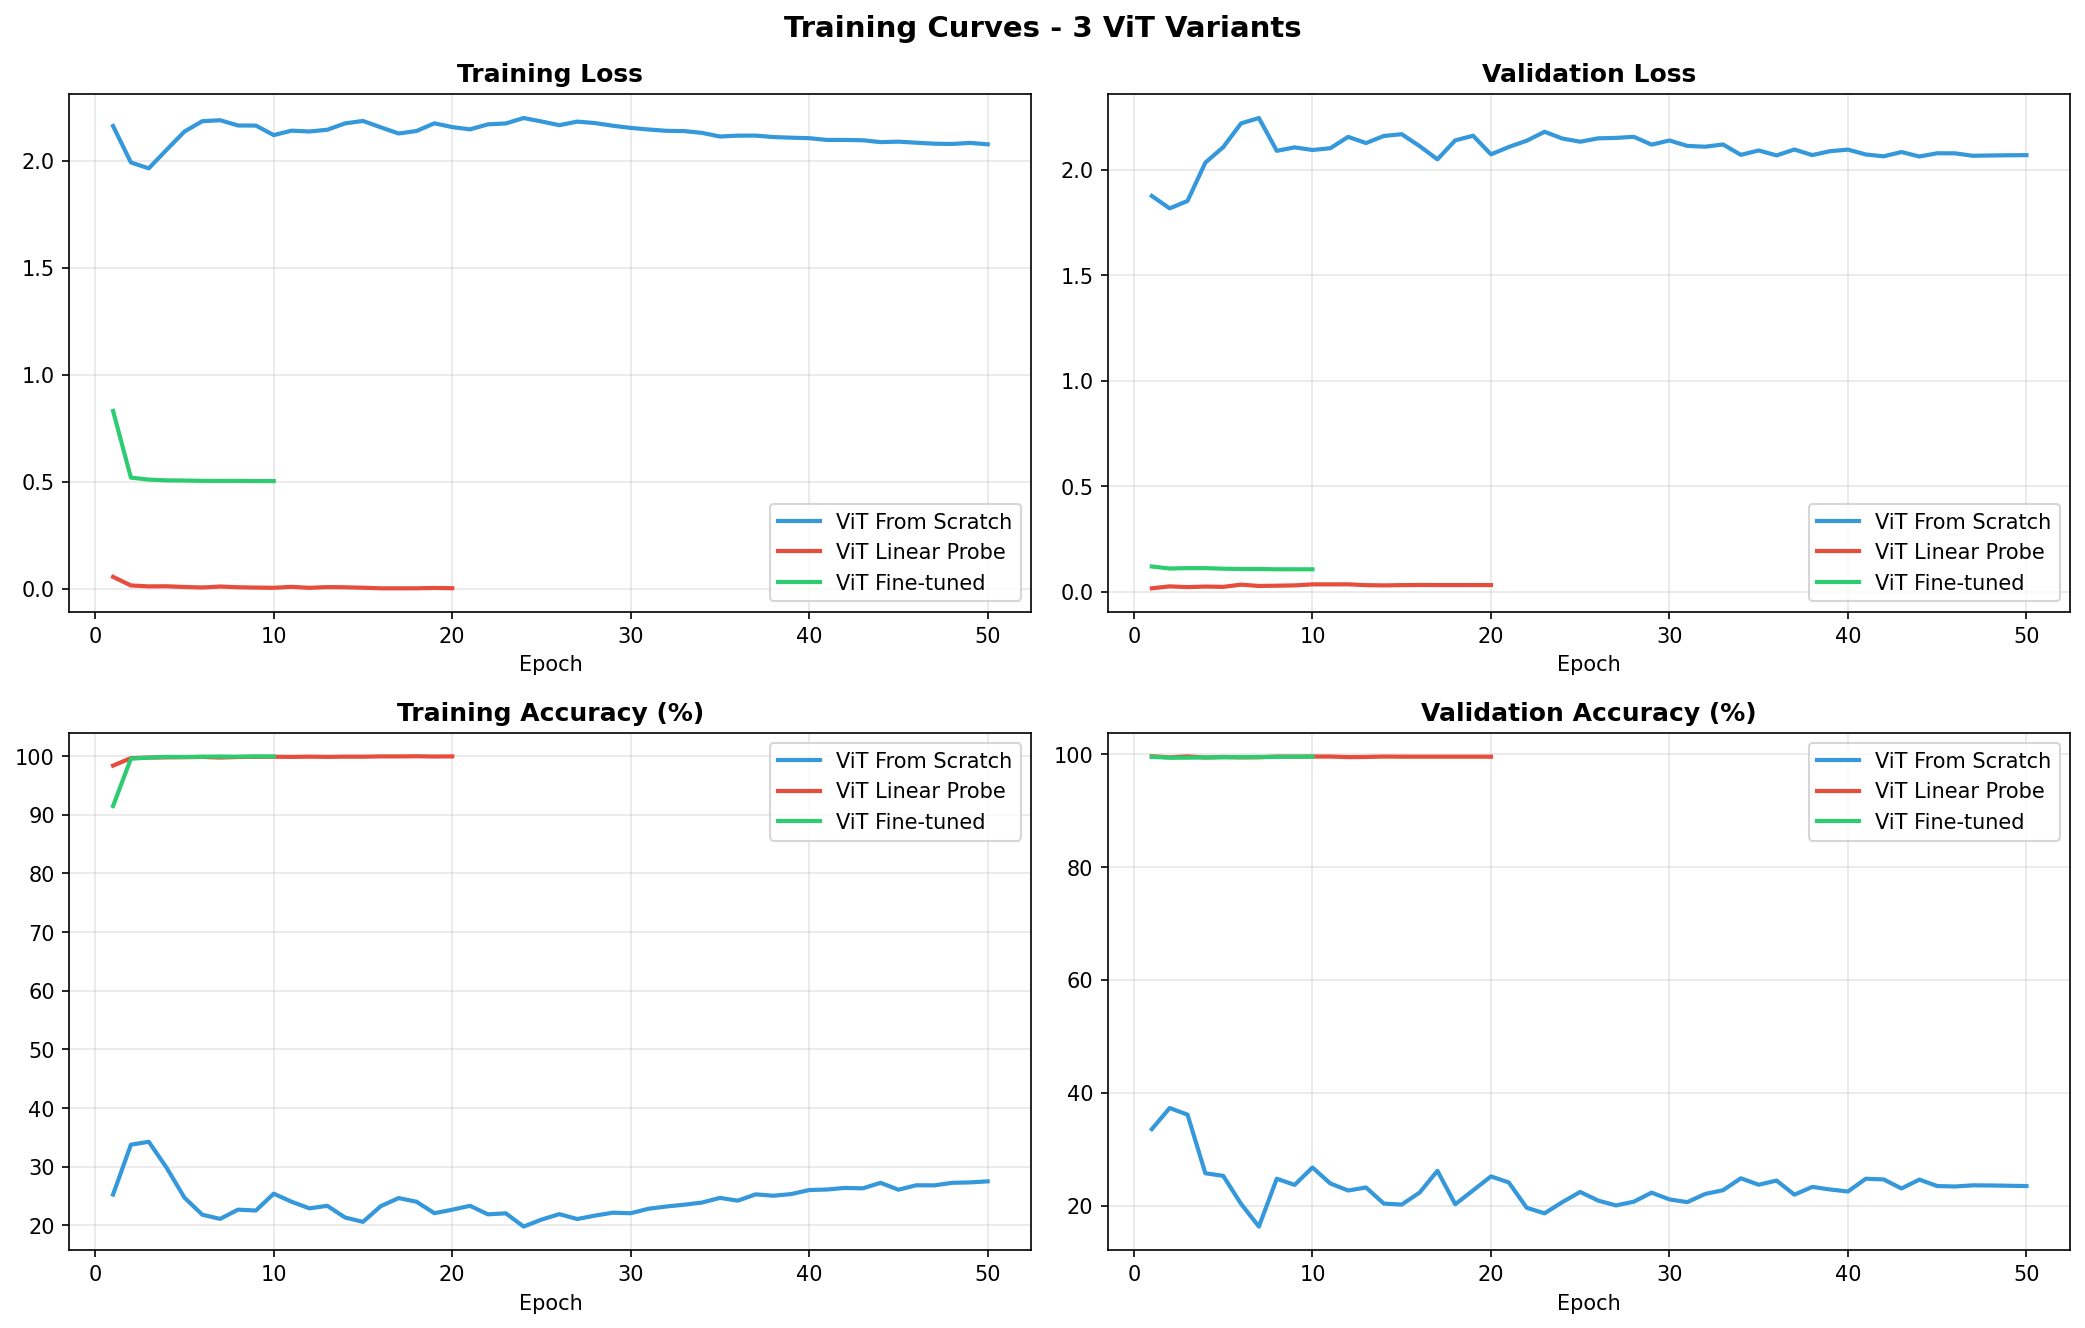
\includegraphics[width=\textwidth]{figures/training_curves.png}
% \caption{Training and validation curves for all three strategies.}
% \end{figure}

The fine-tuned model converged within 10 epochs to 99.59\% accuracy (4.6 min). The linear probe converged even faster, reaching 99.67\% in 20 epochs (4.3 min) while optimizing only 7,690 parameters. The from-scratch model peaked at 37.30\% (epoch 2) but degraded to 23.46\% by epoch 50 (22.6 min), reflecting ViT's difficulty learning from limited data without pretraining.

\subsection{Confusion Matrices and Per-Class Analysis}

%% UNCOMMENT AFTER YOU HAVE FIGURES:
% \begin{figure}[H]
% \centering
% 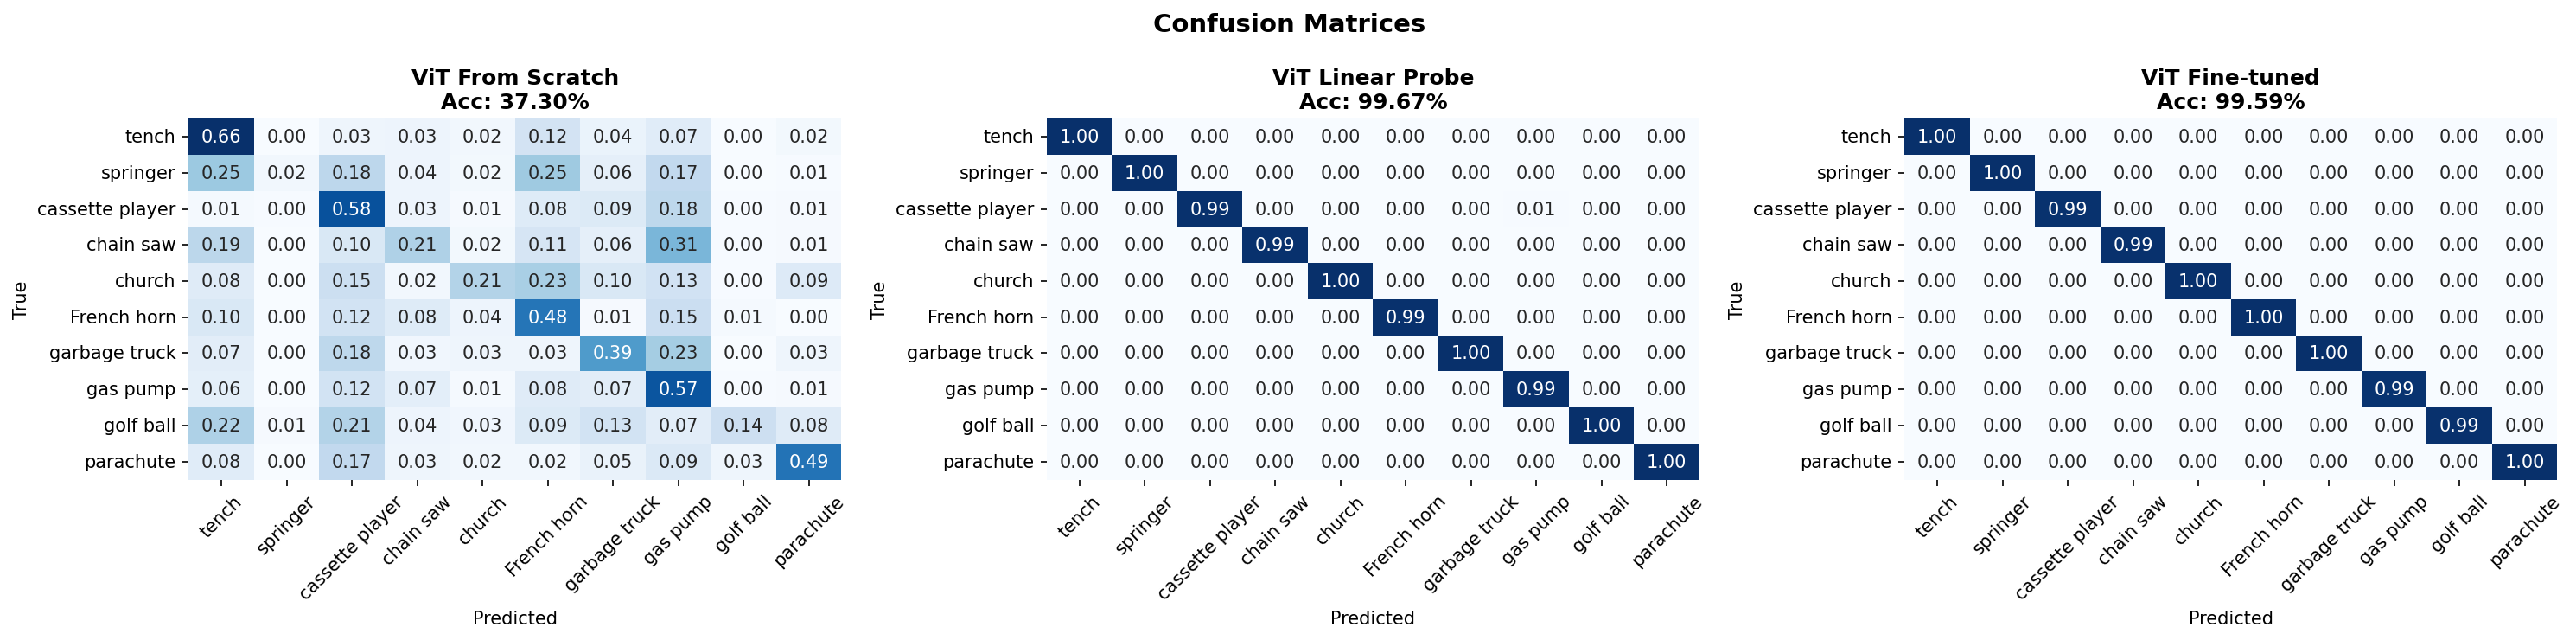
\includegraphics[width=\textwidth]{figures/confusion_matrices.png}
% \caption{Normalized confusion matrices for all three strategies.}
% \end{figure}

The linear probe showed the strongest diagonal (correct predictions) across all 10 classes, closely followed by the fine-tuned model. The from-scratch model exhibited widespread misclassifications across most classes.

\subsection{Attention Map Analysis}

%% UNCOMMENT AFTER YOU HAVE FIGURES:
% \begin{figure}[H]
% \centering
% 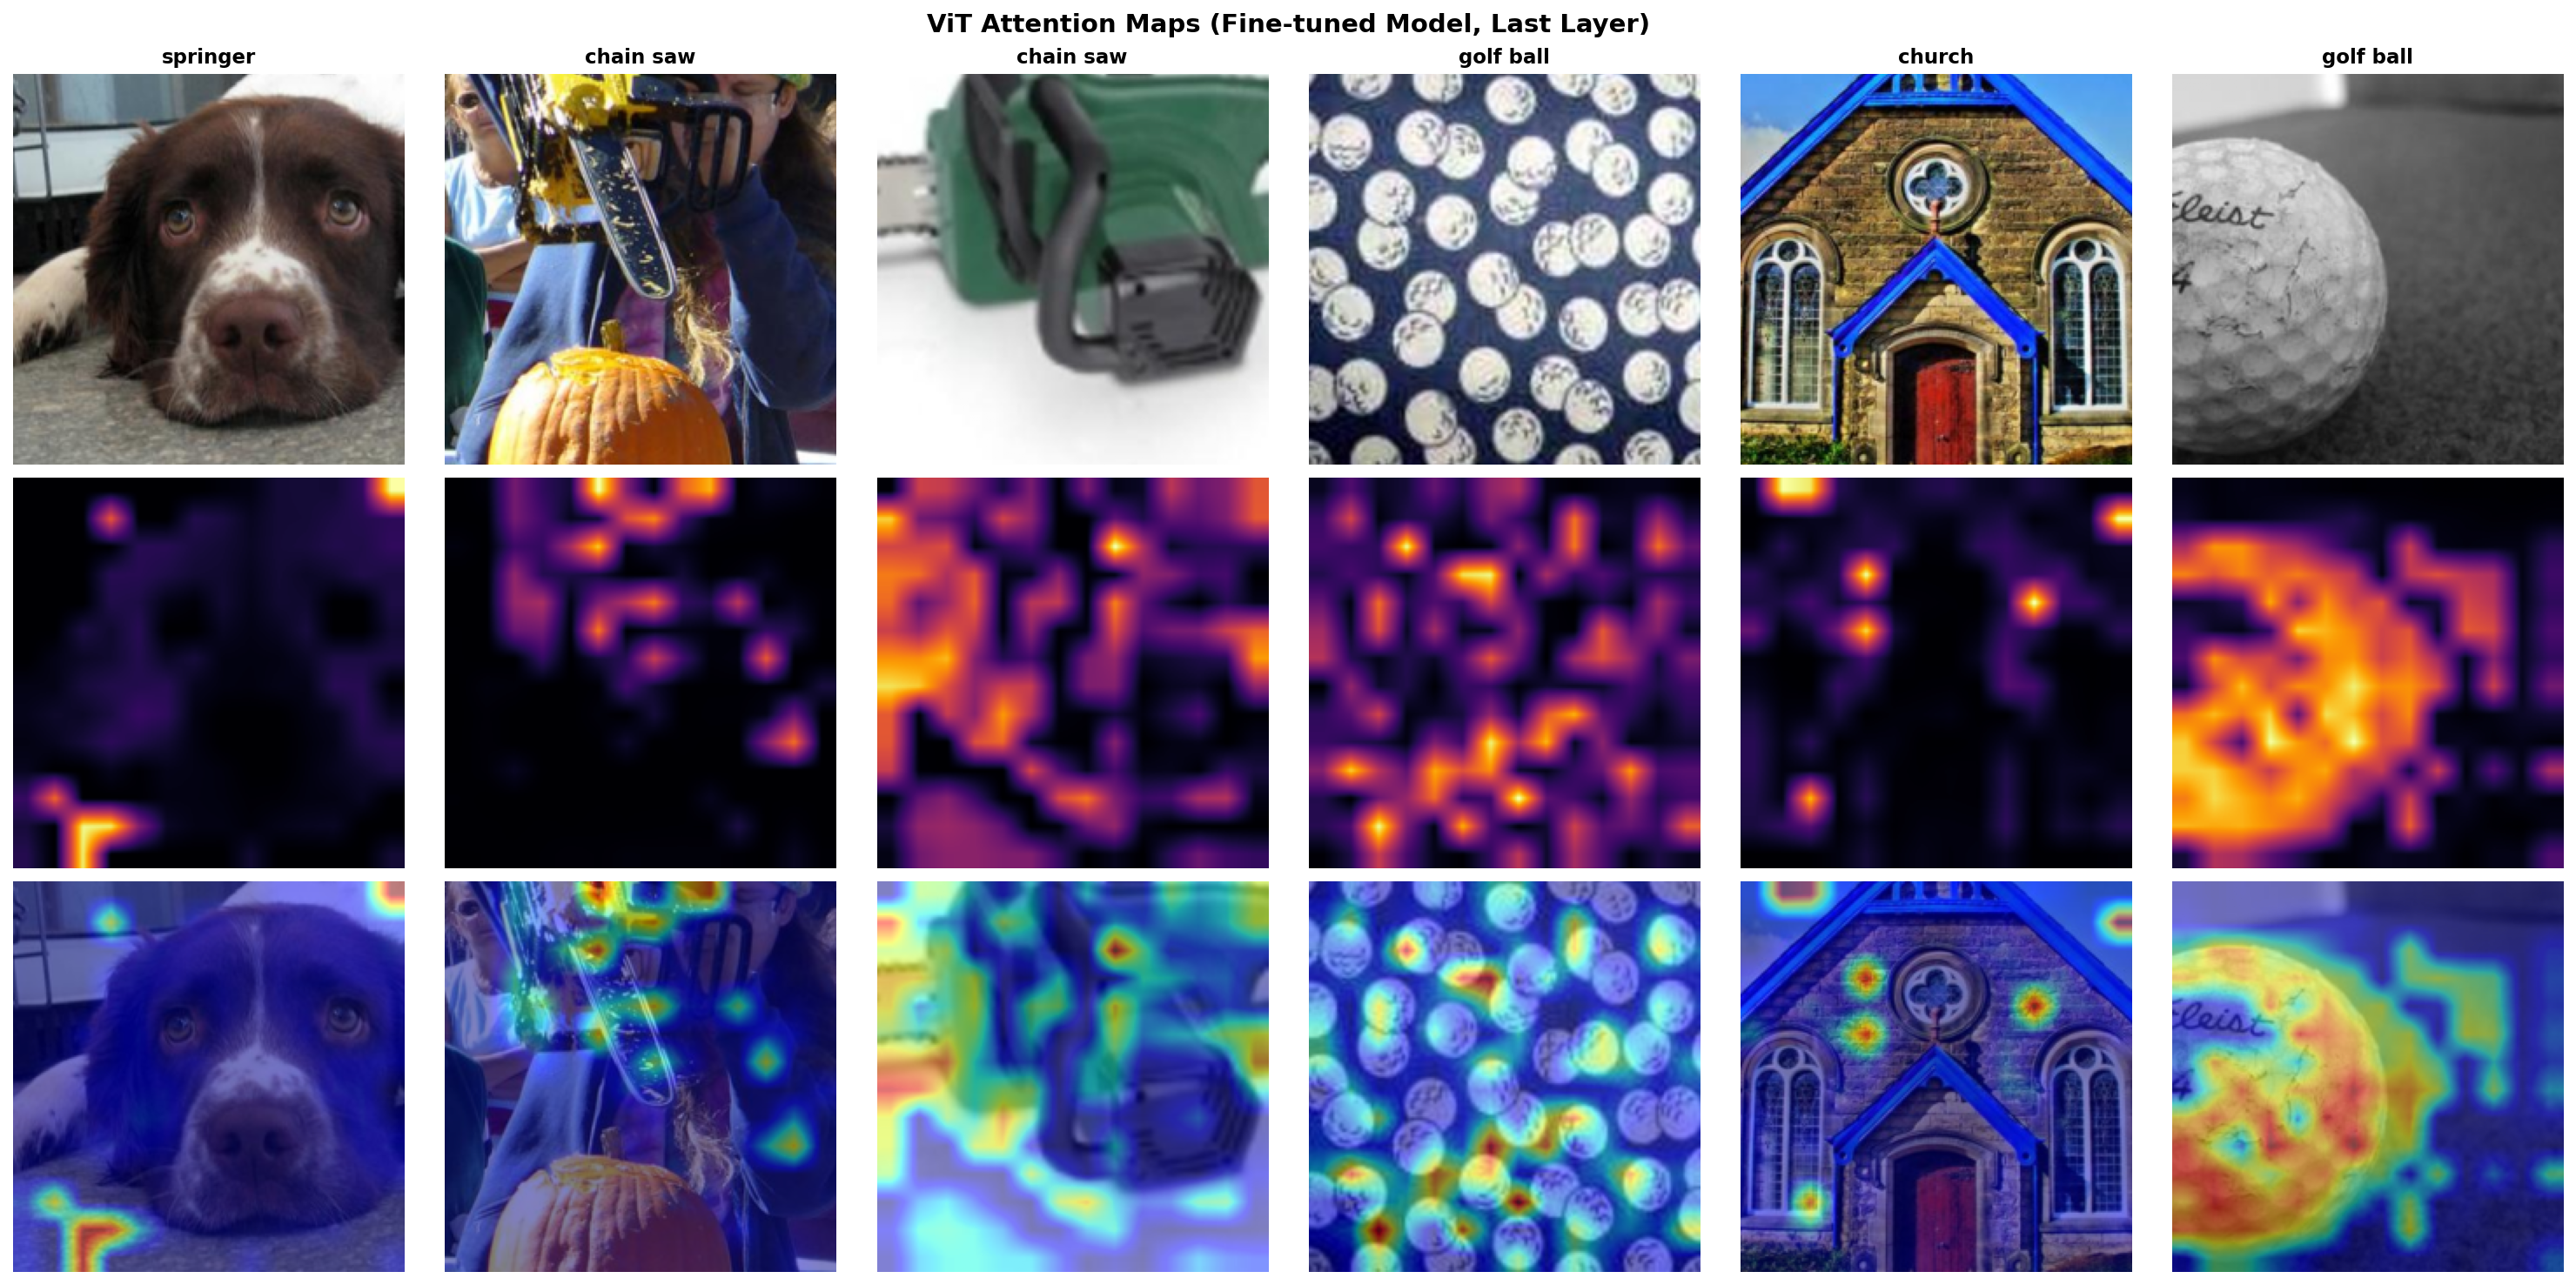
\includegraphics[width=\textwidth]{figures/attention_maps.png}
% \caption{ViT attention maps (fine-tuned model). Top: originals. Middle: attention heatmaps. Bottom: overlays.}
% \end{figure}

The fine-tuned ViT's attention maps show focused attention on semantically relevant object regions. Multi-layer analysis reveals that early layers attend broadly (low-level features) while deeper layers focus on discriminative regions (high-level semantics). Position embeddings demonstrate that ViT learns 2D spatial structure despite receiving patches as a 1D sequence.

% ==============================================================================
% 3. DISCUSSION
% ==============================================================================
\section{Discussion}

\subsection{Why Pretraining Matters for ViT}

The dramatic performance gap between from-scratch and fine-tuned training reveals a fundamental property of Vision Transformers: unlike CNNs, which have built-in inductive biases (locality via small filters, translation equivariance), ViT has no such priors. It must learn spatial relationships entirely from data. With only $\sim$9,500 training images, there is insufficient data for ViT to discover these relationships from scratch.

Pretraining on ImageNet-21k provides the model with rich visual representations learned from millions of images. Even when the backbone is completely frozen (linear probe), these features are powerful enough to achieve 99.67\% accuracy with just 7,690 trainable parameters---in fact surpassing the fully fine-tuned model (99.59\%). This suggests that fine-tuning all 85.8M parameters on a small dataset may introduce slight overfitting, while the frozen backbone provides regularization that preserves the quality of pretrained features.

\subsection{Comparison with Previous CNN/ResNet Study}

\begin{table}[H]
\centering
\caption{Cross-Study Comparison}
\begin{tabular}{lcc}
\toprule
& \textbf{CNN/ResNet (2025)} & \textbf{ViT (2026)} \\
\midrule
Best accuracy & 94.28\% (ResNet-30) & 99.67\% (Linear Probe) \\
Dataset & CIFAR-10 (32$\times$32) & ImageNette (224$\times$224) \\
Key insight & Depth + skip connections & Pretraining is essential \\
Paradigm & Convolutions & Self-attention \\
Interpretability & Limited & Attention maps \\
\bottomrule
\end{tabular}
\end{table}

The previous study showed that architecture design (skip connections) improves CNN performance. This study shows that for transformers, the training strategy---specifically, access to pretrained weights---is the dominant factor. Together, these studies trace the evolution from hand-designed convolutional features to learned attention-based representations.

\subsection{Parameter Efficiency}

The linear probe result is particularly striking: 99.67\% accuracy with only 7,690 trainable parameters (0.009\% of the full model). Not only does linear probing serve as a strong baseline---it actually \textit{outperformed} full fine-tuning (99.67\% vs.\ 99.59\%), suggesting that for datasets closely related to the pretraining domain, unfreezing all parameters may not be necessary and can even be slightly counterproductive.

% ==============================================================================
% 4. CONCLUSION
% ==============================================================================
\section{Conclusion}

This study compared three training strategies for Vision Transformers on ImageNette, yielding the following findings:

\begin{enumerate}
    \item \textbf{Linear probe ViT achieved the best performance} (99.67\%), demonstrating that frozen pretrained features can outperform full fine-tuning on small, domain-similar datasets.
    \item \textbf{Training from scratch fails on small datasets} (37.30\% best at epoch 2, degrading to 23.46\% by epoch 50), confirming that ViT's lack of inductive biases makes pretraining essential.
    \item \textbf{Linear probing outperformed fine-tuning} (99.67\% vs.\ 99.59\% with only 7,690 params---0.009\% of the model), showing that pretrained features transfer exceptionally well and full parameter updates can be unnecessary.
    \item \textbf{Training strategy matters more than model size:} The same 86M-parameter model performed vastly differently depending on how it was trained.
    \item \textbf{Attention maps provide interpretability} not available in traditional CNNs.
\end{enumerate}

\textbf{Limitations:} We tested on one dataset (ImageNette), used a single training run without confidence intervals, and only evaluated ViT-Base. Future work could extend to harder datasets (ImageWoof, full ImageNet), compare model sizes (ViT-Small, ViT-Large), and explore hybrid architectures (Swin Transformer, ConvNeXt).

These results, combined with our previous CNN/ResNet study, illustrate the rapid evolution of computer vision: from convolutional architectures where \textit{design} was key, to transformer models where \textit{pretraining} is everything.

% ==============================================================================
% REFERENCES
% ==============================================================================
\begin{thebibliography}{9}
\bibitem{dosovitskiy2020} Dosovitskiy, A., et al. (2020). \textit{An Image is Worth 16x16 Words: Transformers for Image Recognition at Scale.} arXiv:2010.11929.
\bibitem{he2016} He, K., et al. (2016). \textit{Deep Residual Learning for Image Recognition.} CVPR 2016.
\bibitem{vaswani2017} Vaswani, A., et al. (2017). \textit{Attention Is All You Need.} NeurIPS 2017.
\bibitem{lei2025} Lei, J. (2025). \textit{Comparative Analysis of CNN and ResNet Architectures for CIFAR-10 Image Classification.} MSCS 2202, Sofia University.
\bibitem{howard2020} Howard, J., et al. (2020). \textit{ImageNette: A subset of ImageNet for fast prototyping.} fast.ai.
\end{thebibliography}

\end{document}
